\section{Représentation informatique d'une image}
 
En plus des bibliothèques habituelles
\begin{python}
import numpy as np
import matplotlib.pyplot as plt
\end{python}
on charge la bibliothèque~:
\begin{python}
import scipy.misc
\end{python}
qui nous permet d'utiliser les instructions~: 
\begin{itemize}
\item 
  \verb#img = scipy.misc.imread(filename)#~: le fichier PNG \verb#filename#
  est converti en tableau numpy et nommé \verb#img#.
\item 
  \verb#plt.imshow(img)#~: comme \verb#plt.plot(...)#, l'affichage de
  \verb#img# est préparé, et sera utilisé par \verb#plt.show()# ou
  \verb#plt.savefig(filename2)#.
\item
  \verb#scipy.misc.imsave(filename2, img)# permet d'enregistrer l'image
  (qui n'est pas un schéma python, n'a pas d'axes, de titre etc.)
\end{itemize}

\begin{remark}
  Avec \texttt{scipy.misc}, les tableaux numpy sont de
  \texttt{dtype} \texttt{uint8}, c'est-à-dire «~entiers non signés
  codés sur 8~bits~», soit $\llbracket 0 , 256\llbracket$. 
\end{remark}


\section{Insertion d'un message secret}

\begin{enumerate}
\item 
  Télécharger le fichier PNG \texttt{sagrada\_familia.png}
  sur le site de la classe. \\
  L'ouvrir avec \texttt{scipy.misc.imread} et l'afficher. On
  appellera \texttt{img} le tableau numpy correspondant.\\
  L'objectif de cet exercice est de modifier très légèrement l'image
  pour y cacher un message secret.

% \begin{figure}[h]
%   \centering
%   \includegraphics[width=.45\textwidth]{../sandbox/manipulation_images/sagrada_familia}
% \end{figure}

\item 
  Déterminer pour l'image \texttt{sagrada\_familia.png}~: la taille, le
  \texttt{dtype} et la couleur du  pixel en position (300,300). 
  % Quelle est la taille théorique du fichier~?
  Est-ce que toutes les valeurs de \texttt{img} sont paires~?

\item 
  On exécute le code suivant~: 

  \begin{python}
img1 = np.copy(img)
img1 -= (img1 % 2)    
  \end{python}
  
  Pour \texttt{img1}, préciser la couleur du pixel en position (300,300).\\
  Expliquer le code proposé, et afficher l'image correspondant à
  \texttt{img1}. Que penser~?

\item 
  On définit la fonction suivante~: 

  \begin{python}
def codebinaire(c):
    """Pour un caractère, renvoie son code binaire sur 8 bits
    sous la forme d'un tableau numpy de zéros et uns de longueur 8"""
    # conversion du caractère en son code ascii entier
    x = ord(c)                   # ex : 97 dans le cas de la lettre 'a'
    # conversion de l'entier en binaire
    y = bin(x)                   # ex : '0b1100001'
    # suppression des deux premiers caractères
    z = y[2:]                    # ex : '1100001'
    # ajouts de zéros en début
    t = '0'*(8 - len(z)) + z     # ex : '01100001'
    
    return np.array([int(b) for b in t])    
  \end{python}

  ainsi que le message~: 

  \begin{python}
message = """Le danger réel n'est pas que les ordinateurs commencent à penser comme les humains,
mais que les humains commencent à penser comme des ordinateurs. 
(Sydney Harris)"""    
  \end{python}

  À chaque caractère de la chaîne \texttt{message}, on fait
  correspondre grace à la fonction \texttt{codebinaire} une
  suite de 8 zéros et uns. 

  On décide de cacher le message dans l'image en parcourant
  simultanément les caractères de \texttt{message} et les
  éléments du tableau \texttt{img1} par groupes de~8, et en
  ajoutant respectivement à ces éléments les~8 zéros ou uns
  correspondant au caractère. 

  Implanter cet algorithme et enregistrer le résultat dans un fichier
  \verb#sagrada_avec_message.png#.

\item 
  Quelle est la taille maximale du message que l'on peut cacher par
  cette méthode. 
\end{enumerate}


\section{Décodage d'un message secret}

\begin{enumerate}[resume*]
\item 
  Télécharger le fichier PNG \texttt{traboule\_avec\_message.png}
  sur le site de la classe. L'ouvrir avec \texttt{scipy.misc.imread} et l'afficher. On
  appellera \texttt{img} le tableau numpy correspondant.

% \begin{figure}[h]
%   \centering
%   \includegraphics[width=.45\textwidth]{../sandbox/manipulation_images/traboule_avec_message}
% \end{figure}

\item 
  Déterminer pour l'image \texttt{traboule\_avec\_message.png}~: la taille, le
  \texttt{dtype} et la couleur du  pixel en position (300,300). 

\item 
  Un message a été caché dans cette image, en utilisant le principe
  décrit dans la section précédente. Découvrir ce message. \\
  On précise que \verb#chr(n)# renvoie le caractère codé en
  \textsc{ascii} par l'entier~$n$. Il s'agit donc de la réciproque de
  la fonction \verb#ord(c)#.

\item 
  Indiquer quelques avantages et inconvénients de cette méthode pour
  cacher des messages. 
\end{enumerate}




\begin{figure}[h]
  \centering
  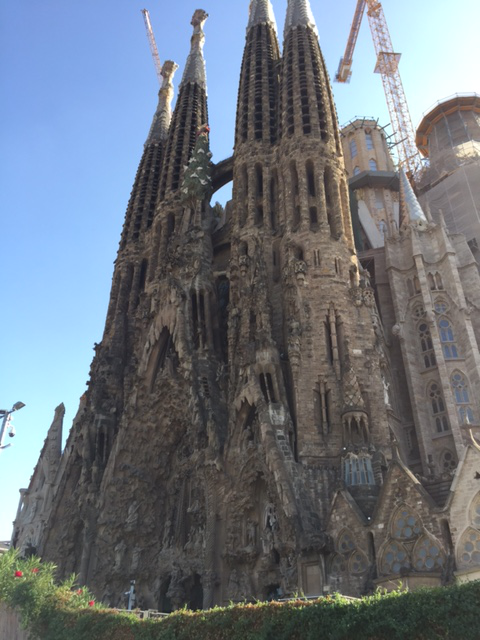
\includegraphics[width=.3\textwidth]{../input_exos_python/theme_image_2_sagrada_familia}
  \hspace*{.1\textwidth}
  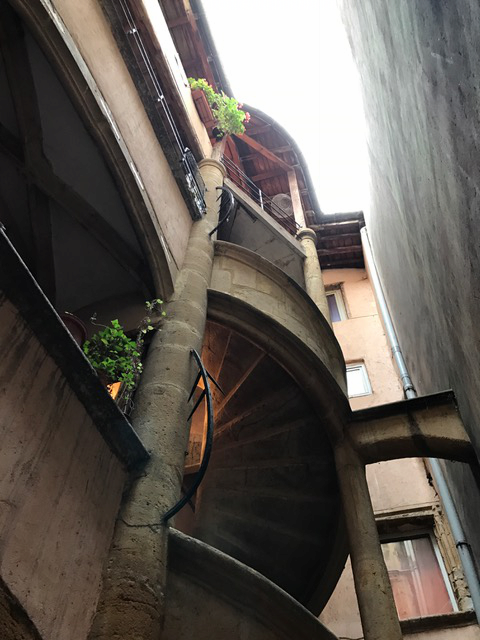
\includegraphics[width=.3\textwidth]{../input_exos_python/theme_image_2_traboule_avec_message}
\end{figure}

